\begin{enumerate}[label=\thesubsection.\arabic*.,ref=\thesubsection.\theenumi]
\numberwithin{equation}{enumi}
\numberwithin{figure}{enumi}


\item   Fig. \ref{fig:ee18btech11025} shows  the Bode magnitude and phase plots of 
    \begin{equation}  
            G(s) = \frac{n_0}{s^3 + d_2 s^2 + d_1 s + d}
    \end{equation}
\begin{figure}[ht!]
        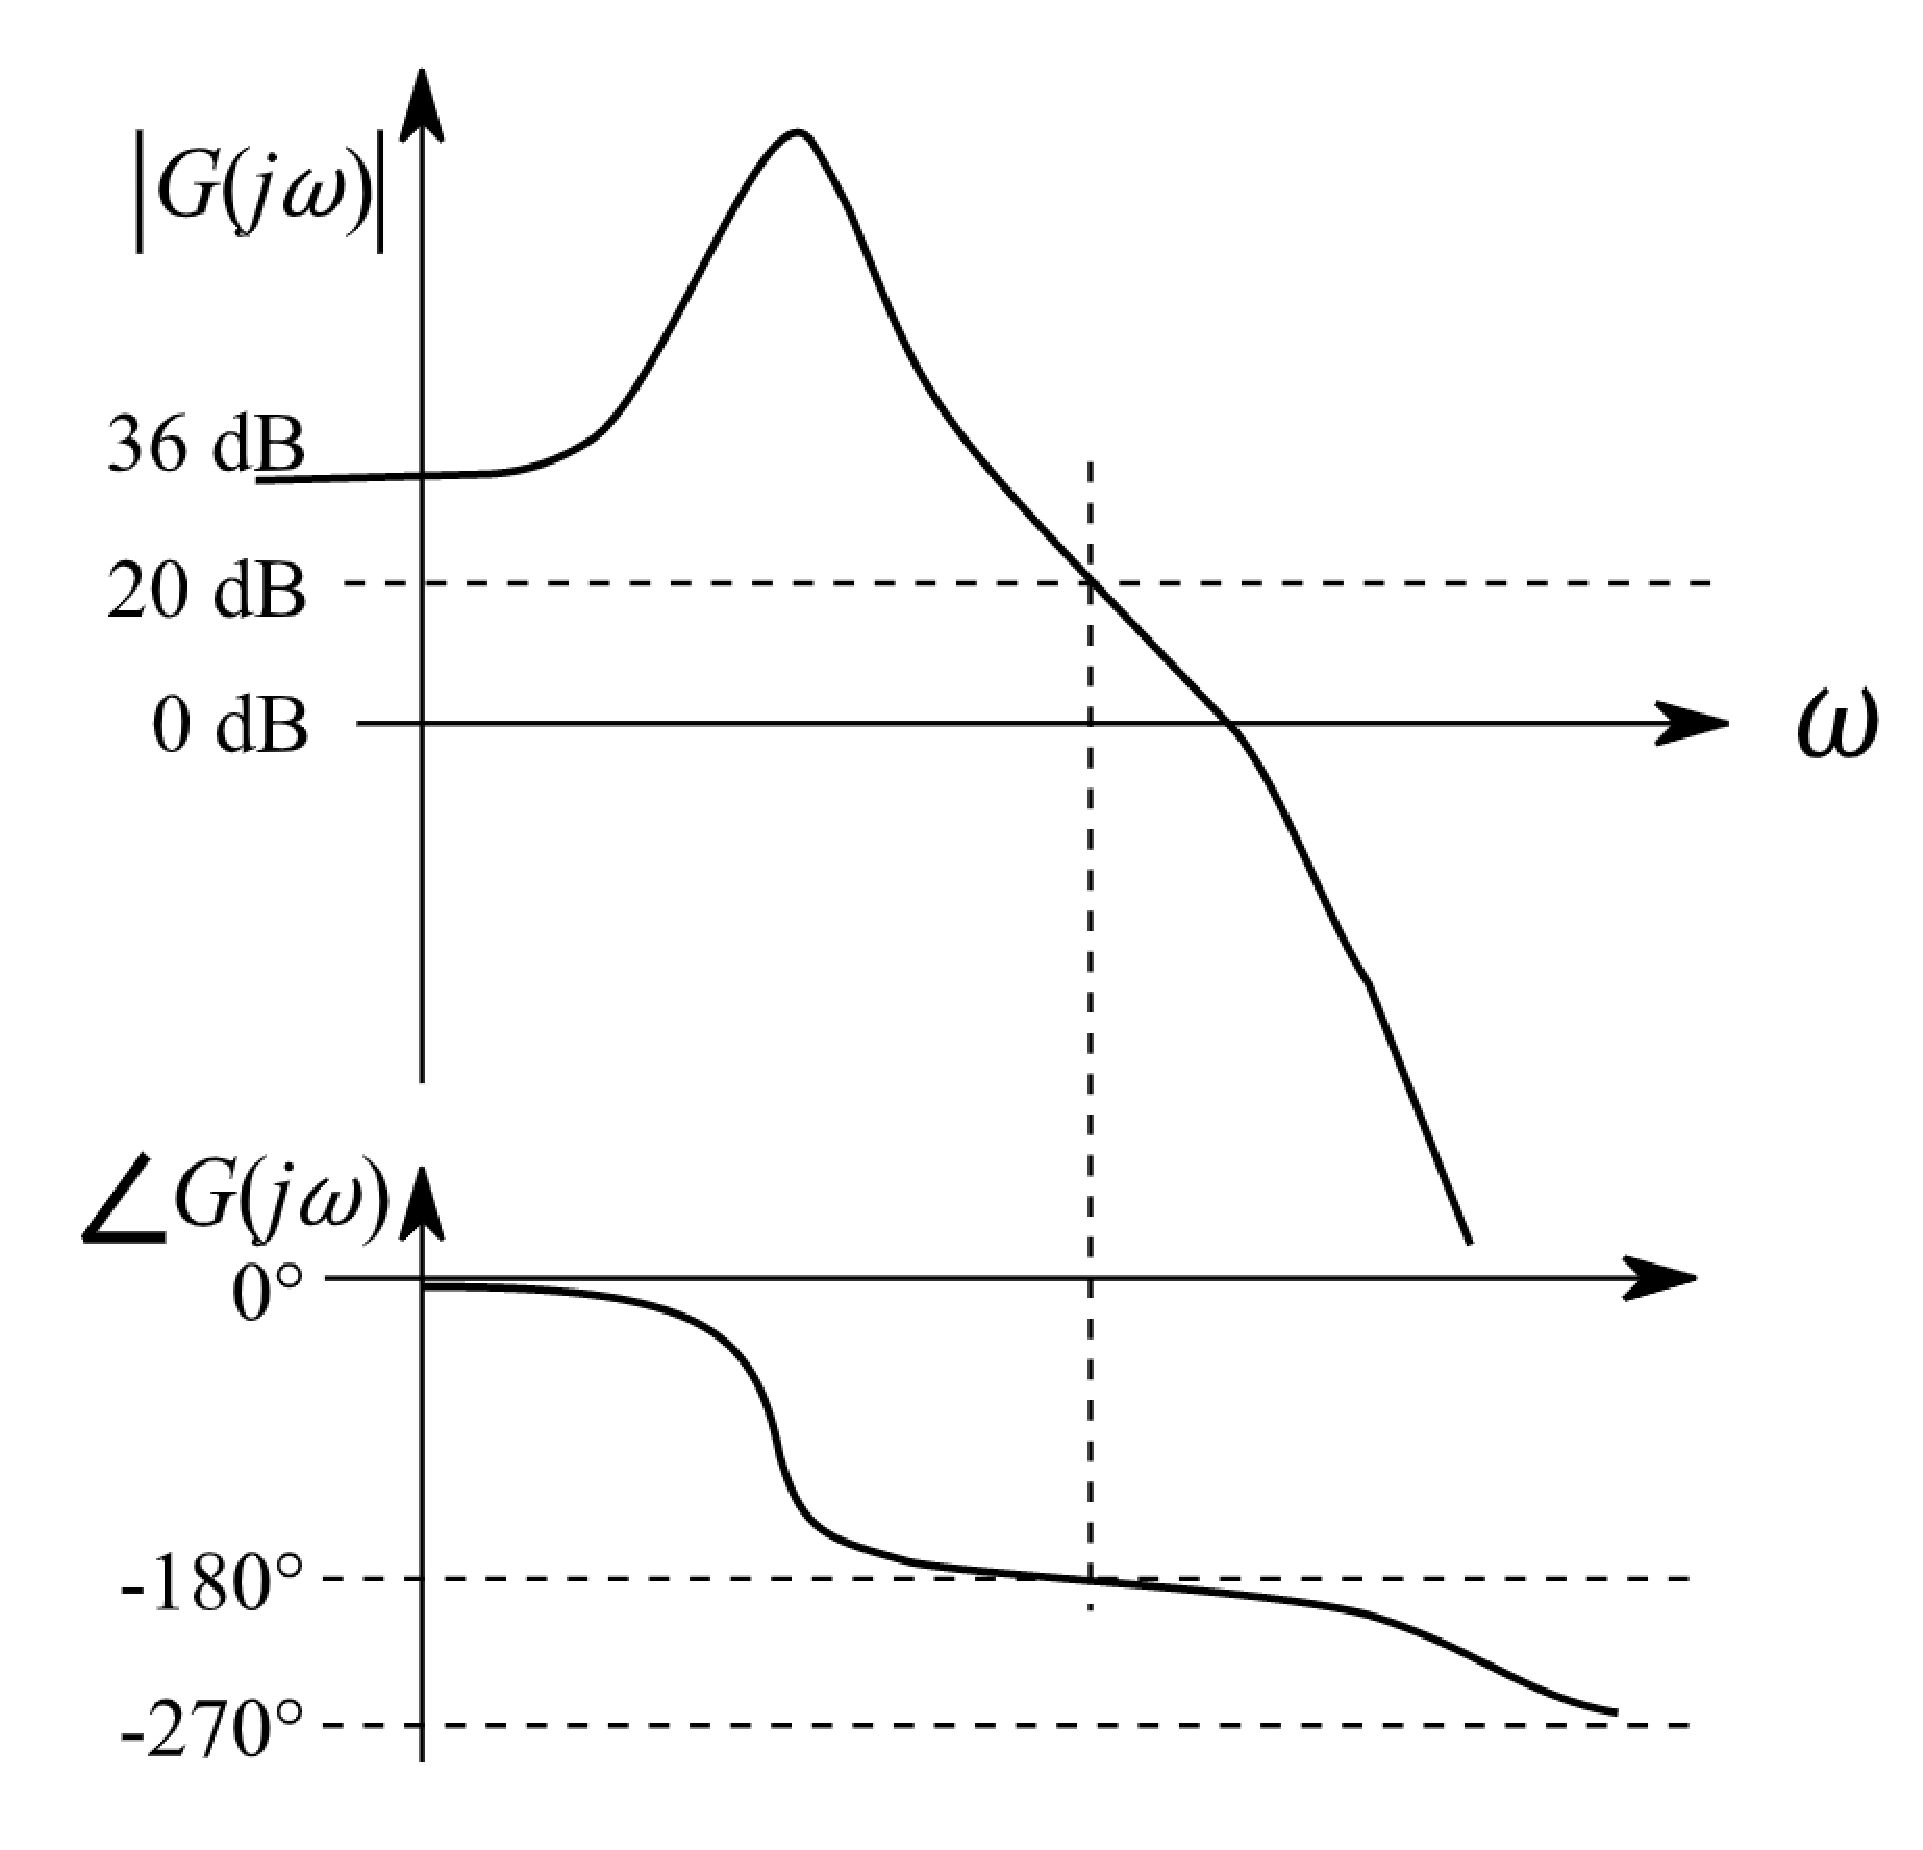
\includegraphics[width=\columnwidth]{./figs/ee18btech11025/q42_1.eps}
        \caption{}
        \label{fig:ee18btech11025}
\end{figure}
Find  $\abs{G\brak{\j\omega_{pc}}}$.
\\
\solution From Fig. \ref{fig:ee18btech11025}, 
%
\begin{align}
\angle G\brak{\j\omega_{pc}}  &= 180 \degree
\\
\implies 20\log\abs{ G\brak{\j\omega_{pc}}}  &= 20
\label{ee18btech11025_g_gain}
%
\end{align}
%


\item  Consider the negative unity feedback configuration with gain $k$ in the feed forward path as shown in Fig.     \ref{fig:ee18btech11025_bock}.  Find the condition for the closed loop system to be stable.
%
\begin{figure}[h]
 \centering
     \resizebox{\columnwidth}{!}{
\tikzstyle{block} = [draw, fill=white!20, rectangle, 
    minimum height=3em, minimum width=4em]
\tikzstyle{sum} = [draw, fill=white!20, circle, node distance=1cm]
\tikzstyle{input} = [coordinate]
\tikzstyle{output} = [coordinate]
\tikzstyle{pinstyle} = [pin edge={to-,thin,black}]
\begin{tikzpicture}[auto, node distance=2cm,>=latex']
    % We start by placing the blocks
    \node [input, name=input] {};
    \node [sum, right of=input] (sum) {$\sum_{}^{}$};
    \node [block, right of=sum] (controller) {$k$};
    \node [block, right of=controller,
            node distance=2.5cm] (system) {G(s)};
    % We draw an edge between the controller and system block to 
    % calculate the coordinate u. We need it to place the measurement block. 
    \draw [->] (controller) -- node[name=u] {} (system);
    \node [output, right of=system] (output) {};
    \coordinate [below of=u] (tmp);

    % Once the nodes are placed, connecting them is easy. 
    \draw [draw,->] (input) -- node {$ $} (sum);
    \draw [->] (sum) -- node {$ $} (controller);
    \draw [->] (system) -- node [name=y] {$ $}(output);
    \draw [->] (input) -- node{$ $} node[pos=0.93]{$+$} (sum);
    \draw [->] (y) |- (tmp) -| node[pos=0.99] {$-$} 
        node [near end] {$ $} (sum);
\end{tikzpicture}
}
    \caption{}
    \label{fig:ee18btech11025_bock}
\end{figure}
\\
\solution The open loop gain for the system in    Fig.  \ref{fig:ee18btech11025_bock} is
%
    \begin{align}  
            G_1(s) &= kG(s)
\\
\implies \angle G_1\brak{\j\omega_{pc}}  &= \angle G\brak{\j\omega_{pc}}  
\\
&= 180 \degree \quad \text{and}
\\
 20\log\abs{ G_1\brak{\j\omega_{pc}}}  &= 20\log \abs{k }+20\log\abs{ G\brak{\j\omega_{pc}}}
\\
&= 20 \brak{1 + \log \abs{k }}
\label{ee18btech11025_g1_gain}
    \end{align}
from \eqref{ee18btech11025_g_gain}.  From \eqref{eq:ee18btech11016_gm_def} and \eqref{ee18btech11025_g1_gain}, the GM of $G_1(s)$ is
    \begin{align}  
-20\log \abs{ G_1\brak{\j\omega_{pc}}} &= -20 \brak{1 + \log \abs{k }}
    \end{align}
%
For stability, $GM > 0$
    \begin{align}  
\implies  -20 \brak{1 + \log \abs{k }} &> 0
\\
\implies  \abs{k} &< 0.1
    \end{align}
%

\end{enumerate}
